Форвард калориметр находится ближе всего к пучку и обеспечивает электромагнитную и адронную калориметрию в диапазоне $3,2 < |\eta| < 4.9$. Из-за своего расположения он подвергается очень сильному воздействию дозы облучения мощностью до $10^6$ ${^\text{Гр}} / _\text{год}$ и потока нейтронов с кинетической энергией более 100 кэВ до 109 $\text{см}^{-2}\text{c}^{-1}$\parencite{tdr_old}. С учётом этих условий форвард калориметр разрабатывался с использованием следующих принципов:
\begin{itemize}
    \item механическая простота с применением небольшого набора материалов;
    \item использование радстойких материалов;
    \item использование материалов с высоким значением Z;
    \item достижение максимальной проективной толщины (вдоль проективных лучей от точки столкновения частиц);
    \item достижение максимальной средней плотности.
\end{itemize}\par
Калориметр состоит из трёх модулей: электромагнитного и двух адронных. В электромагнитной секции в качестве материала адсорбера используется медь, тогда как в адронных -- вольфрам. Номинальные внешние размеры у всех трёх модулей равные. Внутренняя структура представляет собой матрицу шестигранных трубок, расположенных вдоль пучка и изготовленных из материала поглотителя, в которые концентрично установлены медные электроды (рис. \ref{fig:f_cal_struct}). Пространство между стенками трубок и электродами заполнено жидким аргоном, выполняющим роль активного вещества. Конструкция позволяет точно контролировать зазор между электродами.
\begin{figure}[ht]
    \centering
    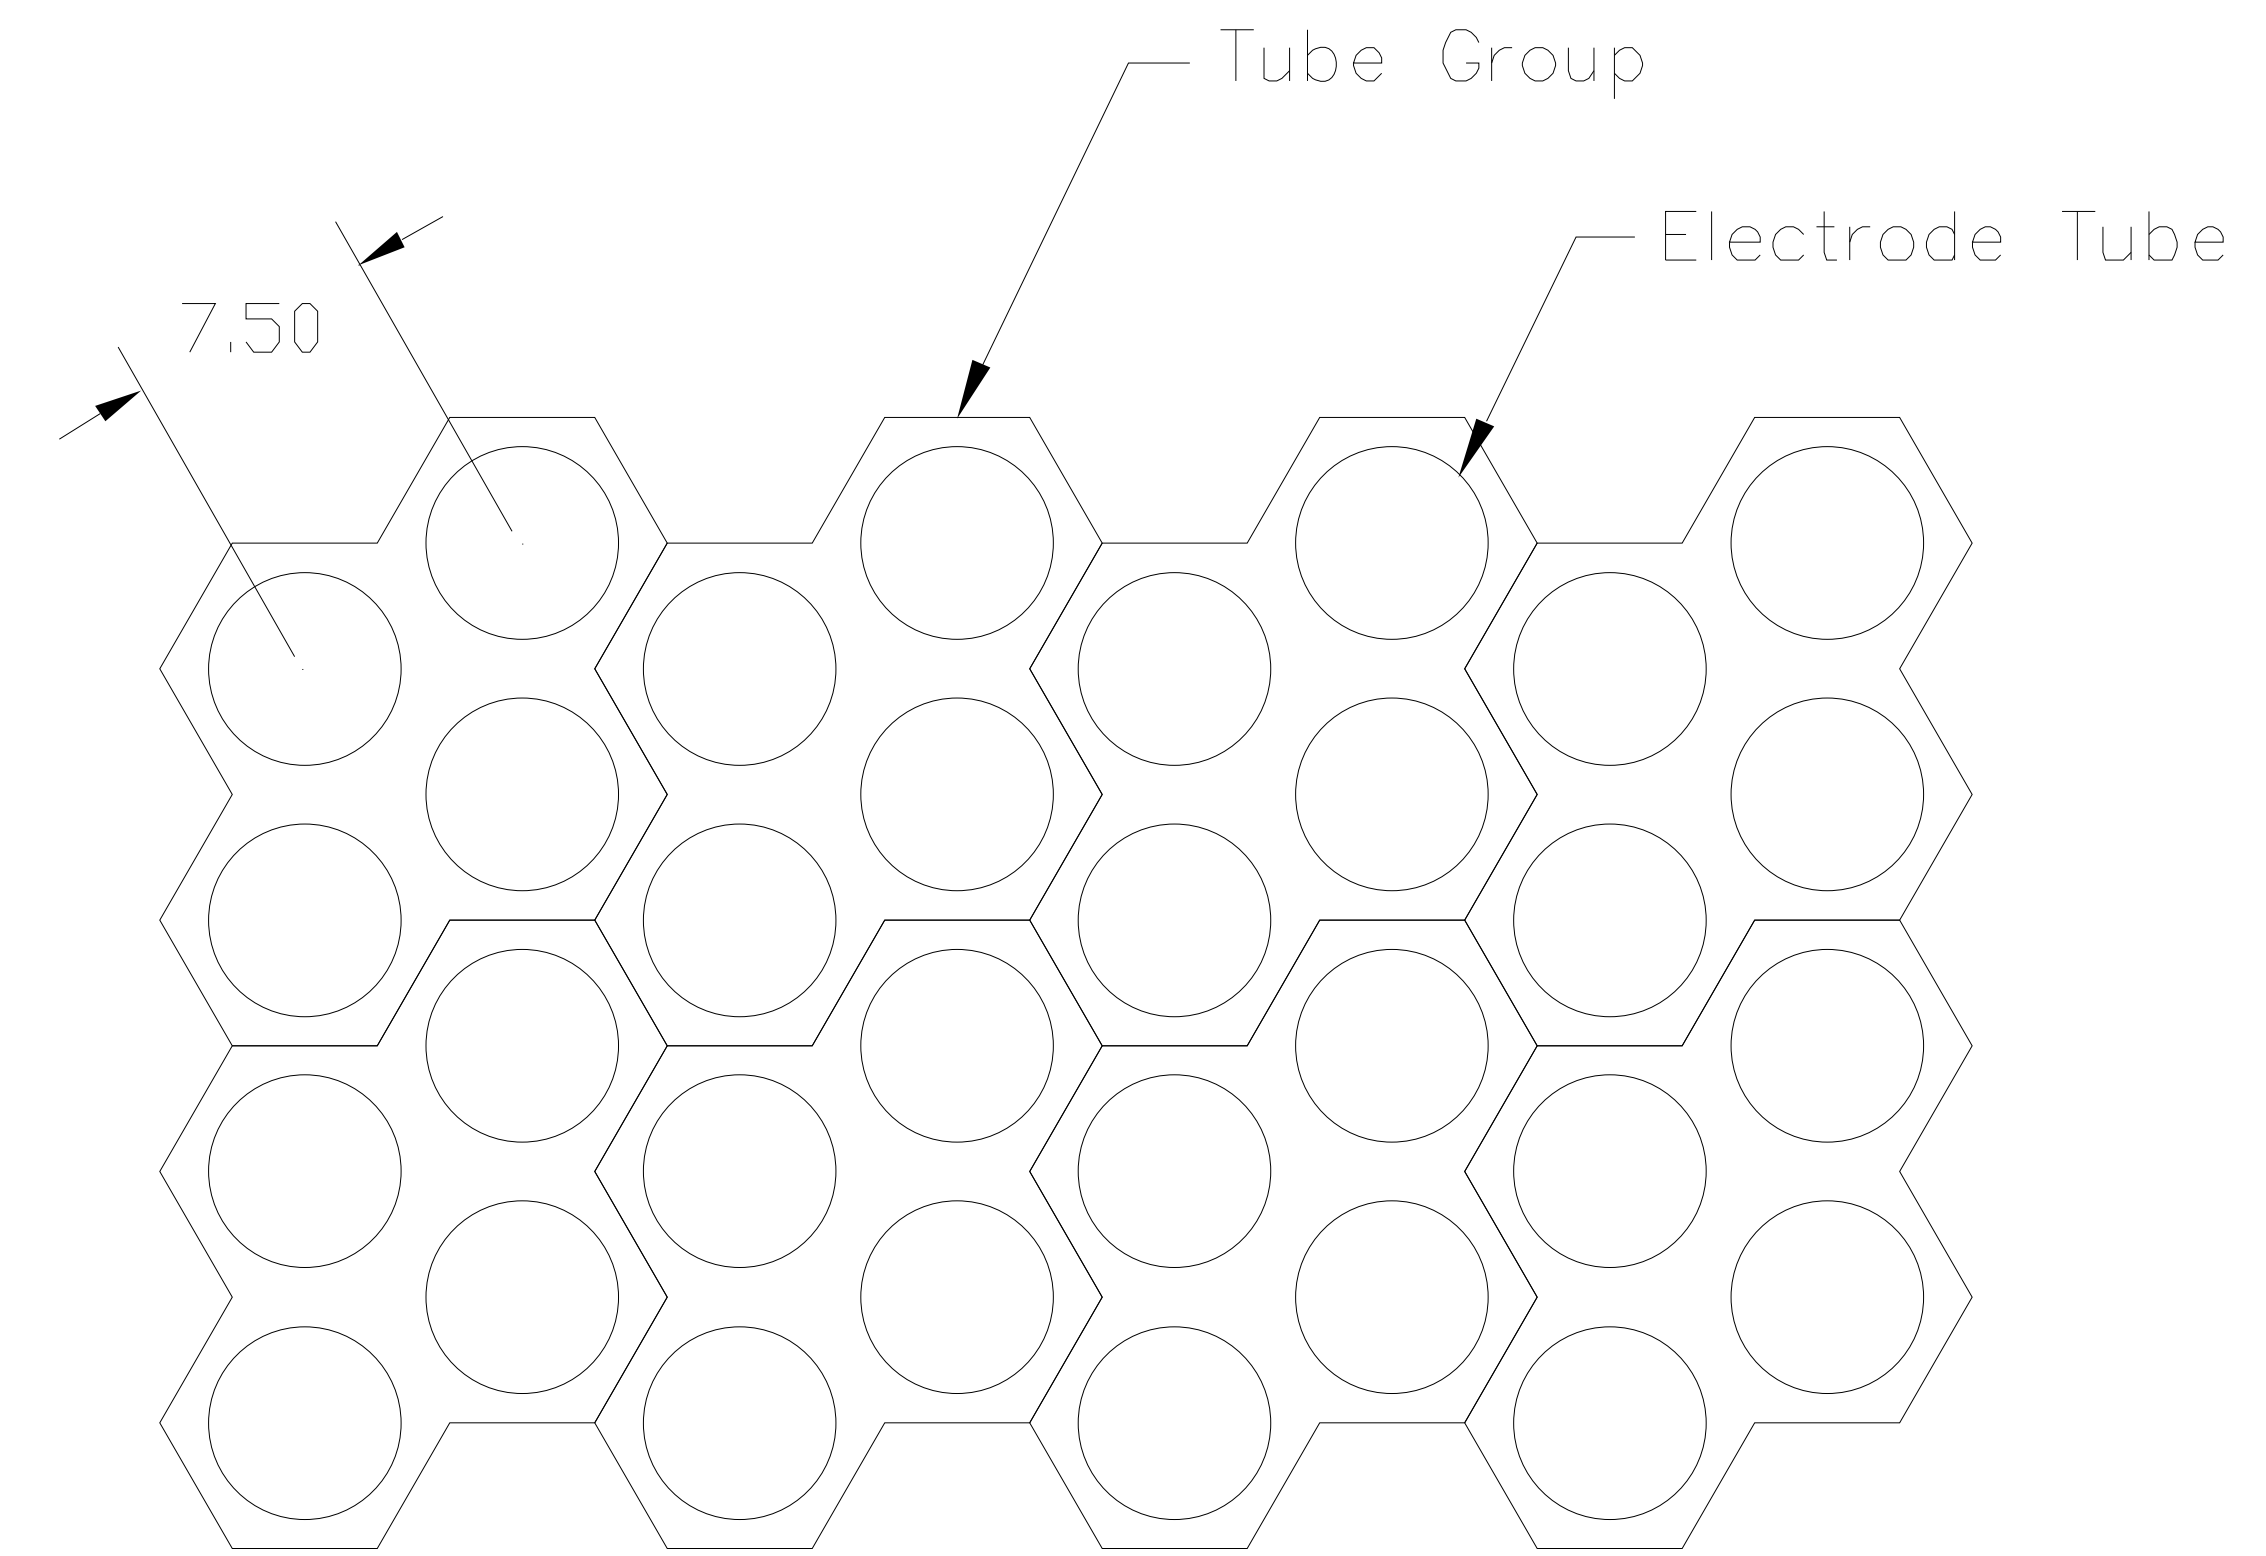
\includegraphics[width=0.6\linewidth]{f_cal_struct.png}
    \caption{Схема внутренней структуры форвард калориметра\parencite{tdr_old}}
    \label{fig:f_cal_struct}
\end{figure}\par
Таким образом, форвард калориметр способен работать в крайне радиационно нагруженных условиях, но при этом имеет сравнительно низкое разрешение. Однако, учитывая тот факт, что проходящие через него частицы имеют одни из наибольших абсолютных энергий, относительная точность остаётся достаточно высокой и такого разрешения вполне хватает для решения существующих физических задач.
